\chapter{Population Synthesis}\label{ch:synthesis}
    In order to derive meaningful conclusions about the outflows from NS mergers, given
    the models described in \ref{ch:introduction}, it was necessary to carry out
    population synthesis studies. In these, population models which are physically or
    observationally motivated are taken from the literature and used to compute the
    statistical properties of the outflows from NS mergers created with these
    properties. If no confident or relevant model exists in literature, physically
    motivated ans\"{a}tze are used (see for example, \S\S\ref{sub:spin-dists}).\\
    In each study which uses (slightly) different population models, 10$^5$ samples were
    drawn from the relevant parameter distributions. Using these as inputs the expected
    outflows were calculated using the fit formulae described in
    \ref{ch:introduction}.\\
    In this chapter, the various population models are briefly described along with
    their pertinence. Furthermore, preliminary checks for the population synthesis code
    are also discussed, which help verify the consistency of the code with theoretical
    results.

\section{Black Hole Population Models}\label{sec:bh_pop}

    \subsection{Mass, $M_{BH}$}
        The masses of the black holes was sampled from the `truncated' mass distribution
        from \cite{abbott_2020B}. The distribution `produces' black holes with masses
        between 3--100 M$_\odot$ (as can be seen from Fig.  \ref{fig:bh_mass_gwtc2}).
        However, NS binaries with extremely massive ($M_{BH} > 20 M_\odot$) black holes
        will not produce any appreciable EM emission due to the NS companion plunging
        into the black hole directly without significant tidal disruption. For this
        reason the population synthesis code imposes an upper limit to the black hole
        masses sampled.

        \begin{figure}[H]
            \centering
            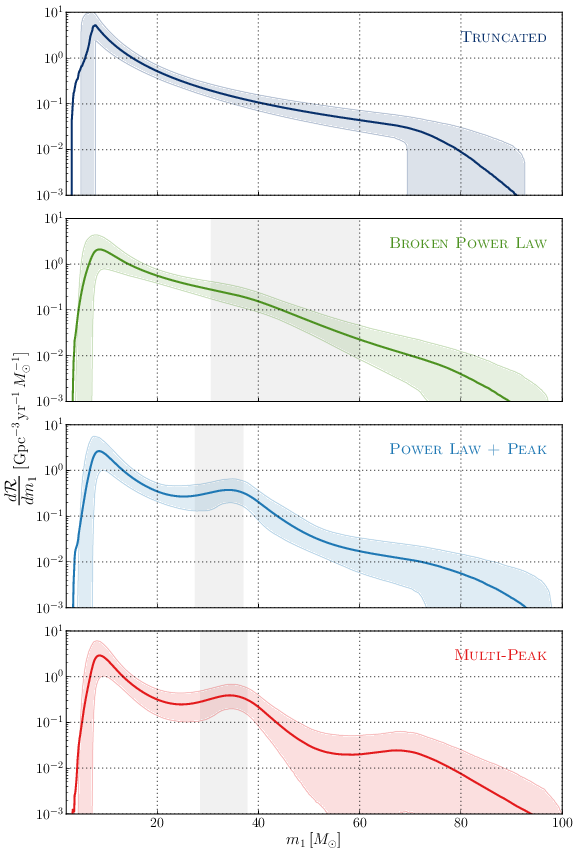
\includegraphics[width=\linewidth]{bh_mass_gwtc2}
            \caption[Black hole mass distributions from GWTC-2]{
                Black Hole Mass Distributions from \cite{abbott_2020B}. In the current
                study the `truncated' mass distribution with an upper limit at 20
                M$_\odot$, since more massive black holes would not produce significant
                EM emission when in a merging NSBH binary.
            }
            \label{fig:bh_mass_gwtc2}
        \end{figure}

        \begin{figure}[H]
            \centering
            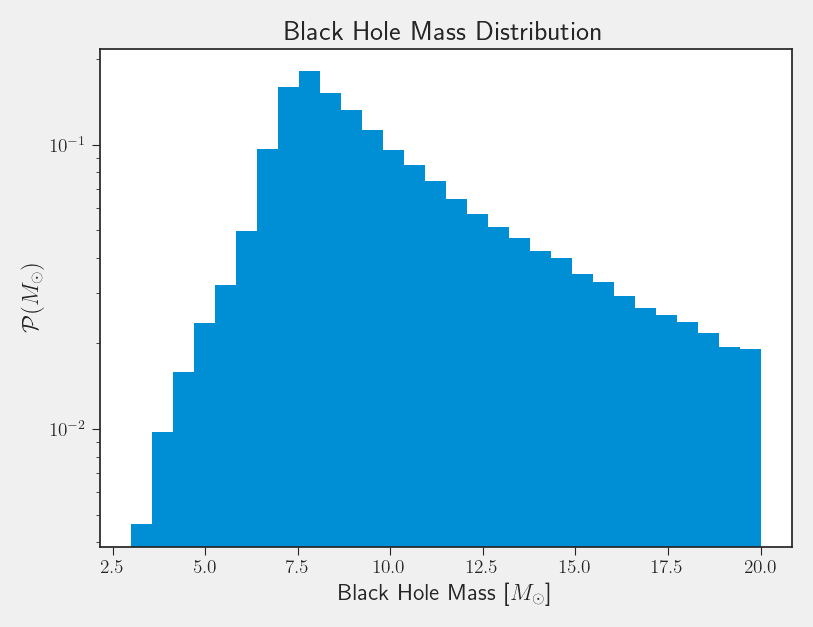
\includegraphics[width=0.8\linewidth]{bh_mass}
            \caption[Black hole mass distribution with upper limit]{
                Black hole mass distribution as used in the current report, with an
                upper limit of 20 M$_\odot$.
            }
            \label{fig:bh_mass}
        \end{figure}

    \subsection{Spin, $chi_{BH}$}\label{sub:spin-dists}
        The spins of the black holes are sampled from the `default' distribution given
        in \cite{abbott_2020B}. This distribution is essentially a Beta distribution
        , which ensures that the spin parameters sampled from this distribution remain
        within [0, 1).\\

        \begin{figure}[H]
            \centering
            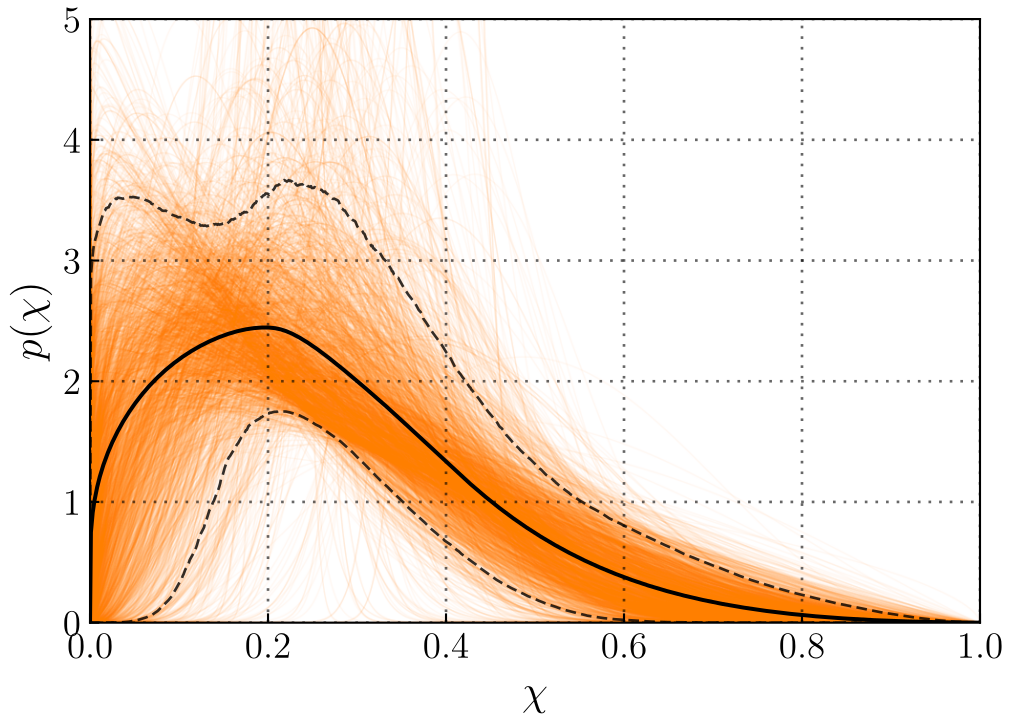
\includegraphics[width=0.8\linewidth]{bh_spin_gwtc2}
            \caption[Black hole spin distribution from GWTC-2]{
                Beta distribution for the  black hole spin from \cite{abbott_2020B}.
                Here the light traces are samples from the posterior distribution,
                whereas the solid black line is the posterior probability distribution
                for $\chi_{BH}$. Dashed black lines mark the 90\% quantiles for the
                same.
            }
            \label{fig:bh_spin_gwtc2}
        \end{figure}

        However, since there have been no confident NSBH merger detections in the GW
        regime, this distribution is largely derived from looking at BBH mergers, and so
        may not represent the true spin distribution of a black hole in a NSBH binary.
        To circumvent this, the following ans\"{a}tze are used to probe the effect of
        the spin distribution on the EM outflows:

        \begin{itemize}

            \item Uniform spin distribution: here $\chi_{BH} \sim \mathcal{U}(0, 1)$.
                Note also that this distribution will have a higher number of high spin
                samples as compared to the `default' distribution considered above.

            \item Gaussian spin distribution: here $\chi_{BH} \sim \mathcal{N}(\mu,
                \sigma)$, but samples outside of [0, 1) are not considered. For
                simplicity and to cover a representative sample of the possible
                distributions, samples were taken from $\mathcal{N}(0.2, 0.2)$,
                $\mathcal{N}(0.5, 0.2)$ and $\mathcal{N}(0.7, 0.2)$. These represent
                distributions concentrated around low, medium and high spins
                respectively.

        \end{itemize}

        % TODO: insert figures for the uniform and gaussian spin distributions!

\section{Neutron Star Population Models}\label{sec:ns_pop}

    In order to reduce the number of variables in the problem, the masses of all neutron
    stars in the population was set to 1.4 M$_\odot$. This value corresponds to the
    median neutron star mass as inferred from GW170817 (see \cite{abbott_2018}). Also,
    the spins of all neutron stars was set to 0, since it is assumed that sufficient
    amount of time would have passed between the formation of the binary and merger,
    allowing for the neutron star to spin down such that $\chi_{NS} \sim 0$.\\
    Additionally, the tidal deformability of the neutron stars was set using the C-love
    relation (see \cite{yagi_2017}). First, the radii of the neutron stars were set to
    11 km, which is the median neutron star radius inferred for GW170817. Then, the
    compactness of the neutron stars, $C_{NS}$ was computed using the relation :

    \begin{equation}
        C_{NS} = \dfrac{G M_{NS}}{R_{NS} c^2}
    \end{equation}

    where $M_{NS}$, $R_{NS}$ are the mass and radius of the neutron star, G is the
    universal gravitational constant and c is the speed of light.  Finally, the tidal
    deformability is computed by solving the C-Love relation :

    \begin{equation}
        C_{NS} = \sum_{k=0}^{2} a_k (\ln \Lambda_{NS})^k
    \end{equation}

    where $\Lambda_{NS}$ is the tidal deformability of the neutron star, and $a_k$ are
    the fit coefficients as given in \cite{yagi_2017}.

\section{Spatial Distribution and Orientation of events}\label{sec:space_dist}

    \subsection{Constant comoving volume distribution}

        The events whose component mass and spin distributions were described in
        \ref{sec:bh_pop}-\ref{sec:ns_pop} are distributed in 3D space such that their
        number density is constant in comoving volume.\\
        For this, firstly the latitudinal ($\theta$) and longitudinal ($\phi$) angles
        are sampled such that $\cos \theta \sim \mathcal{U}(-1, 1)$ and $\phi \in
        \mathcal{U}(0, 2\pi)$, i.e. they are sampled such that they are uniform on a
        unit sphere. As for the comoving distance distribution $\mathcal{P}(D_c)$,
        consider the probability of an event lying in an infinitesimal shell of width
        d$D_c$ at a comoving distance $D_c$.  Then it can be seen that:
        \begin{equation}
            \mathcal{P}(D_c) dD_c \propto D_c^2 dD_c \Rightarrow
                \boxed{\mathcal{P}(D_c) = \alpha D_c^2}
        \end{equation}
        where $\alpha$ is the constant of proportionality. In the local universe, it can
        be safely assumed that $D_c \approx D_L$, where the latter is the luminosity
        distance.  However, from the fact that the GW SNR $\rho \propto D_L^{-1}$ it can
        also be seen that:

        \begin{align}
            \mathcal{P}(\rho) &= \mathcal{P}(D_L)
                                  \Big \lvert \dfrac{dD_L}{d\rho} \Big \rvert \\
                              &= \mathcal{P}{D_c}
                                  \Big \lvert \dfrac{dD_c}{d\rho} \Big \rvert \\
                              &\propto \dfrac{1}{\rho^2} \dfrac{1}{\rho^2}
                                  = \dfrac{1}{\rho^4} \nonumber\\
            \Rightarrow \mathcal{P} (\rho) &= \dfrac{\beta}{\rho^4}
        \end{align}

        Once the SNR detection threshold\footnote{
            This is defined such that any event with a GW network SNR greater than the
            detection threshold will be considered a detection.
        } ($\rho_{th}$) is set, the normalization constants can be computed as follows:

        \begin{align}
            \int_0^{D_{c, max}}
                \mathcal{P}(D_c) dD_c &= \int_0^{D_{L, max}} \mathcal{P}(D_L) dD_L \\
                                      &= \int_0^{\rho_{th}} \mathcal{P}(\rho) d\rho \\
                                      &= 1
        \end{align}

        This gives:

        \begin{align}
            \label{eq:lum_dist}
            \mathcal{P}(D_L) = 3 \dfrac{D_L^2}{D_{L, max}}
                                 \Leftrightarrow
            \mathcal{P}(\rho) = 3 \dfrac{\rho_{th}^3}{\rho^4}
        \end{align}

        where $D_{L, max}$ is the luminosity distance corresponding to the detection
        threshold. As an example, for the Advanced LIGO/VIRGO configuration and a SNR
        threshold of 10, $D_{L, max} \approx 1123$ Mpc.\\
        Using Eq.\ref{eq:lum_dist}, samples are drawn from the luminosity distance
        distribution and using the previous samples for $\theta$ and $\phi$, events are
        distributed in 3D space such that the number density of events is constant in
        the comoving volume.

    \subsection{Orientation of Events}\label{sub:orientation_of_events}

        The orientation of NSBH binaries with respect to the line-of-sight is prescribed
        using the inclination angle, $\iota$ and the polarization angle of the incoming
        GW signal, $\psi$. These are distributed for the population such that $\cos\iota
        \sim \mathcal{U}(-1, 1)$ and $\psi \sim \mathcal{U}(0, 2\pi)$, from which
        samples are drawn for individual events.

\section{Summary}
